\documentclass[english, 11pt, a4paper]{article}
\usepackage{amsmath, amssymb,amsthm}
\usepackage{setspace, natbib}
\usepackage{bm}
\usepackage{threeparttable}
\usepackage{graphicx}
\usepackage{booktabs}
\usepackage{dcolumn}
\usepackage{tabu}
\usepackage{longtable}
\usepackage{float}
\usepackage{caption}
\usepackage{subcaption}
\usepackage[procnames]{listings}
\usepackage{color}
\setlength{\textwidth}{15.5cm} \setlength{\textheight}{22cm}\setlength{\oddsidemargin}{-0.5mm}
\setlength{\parskip}{1ex plus0.5ex minus0.5ex}\setlength{\parindent}{0mm}
\DeclareMathOperator\erfc{erfc}
\usepackage{babel}


\definecolor{keywords}{RGB}{255,0,90}
\definecolor{comments}{RGB}{0,0,113}
\definecolor{red}{RGB}{160,0,0}
\definecolor{green}{RGB}{0,150,0}
 
\lstset{language=Python, 
        basicstyle=\ttfamily\small, 
        keywordstyle=\color{keywords},
        commentstyle=\color{comments},
        stringstyle=\color{red},
        showstringspaces=false,
        identifierstyle=\color{green},
        procnamekeys={def,class}}


\renewcommand{\bibfont}{\footnotesize}
\setlength{\bibsep}{1pt}

\begin{document}

\baselineskip18pt


\title{Order Book Analysis}

\author{Artagan Malsagov}

\date{\today}


\maketitle
%\newpage 
%\tableofcontents

%\section{Introduction}

\section{Data Description}

The data consist of 5 levels of both sides of the order book, for 5 different days.
Each days spans roughly 10 hours worth of data (36 billion micros, see table below)

\begin{table}[H]
    \centering
    \begin{tabular}{lrrrr}
    \toprule
    date & min timestamp & max timestamp & avg bbo mid & avg 5 level order volume \\
    \midrule
    20190610 & 0 & 36000000000 & 10064 & 673 \\
    20190611 & 0 & 36000000000 & 10127 & 866 \\
    20190612 & 0 & 36000000000 & 9999 & 955 \\
    20190613 & 0 & 36000000000 & 10065 & 908 \\
    20190614 & 0 & 35999621354 & 9894 & 797 \\
    \bottomrule
    \end{tabular}
    \label{tab2}
\end{table}


\subsection{Data resampling}
The order book is of the form below:

\begin{table}[H]
    \centering
    \begin{tabular}{crrrr}
    \toprule
    timestamp & bp0 & bq0 & ap0 & aq0 \\
    \midrule
    110 & 10045& 62 & 10055 & 98 \\
    175 & 10065& 46 & 10075 & 42 \\
    220 & 10075& 9 & 10080 & 25 \\
    \bottomrule
    \end{tabular}
    \label{tab2}
\end{table}

where the timestamps are in microseconds. Plotting a histogram of the frequency of the timestamps,
we see that the updates aren't uniformly distributed: 

 \begin{figure}[H] 
	\centering
	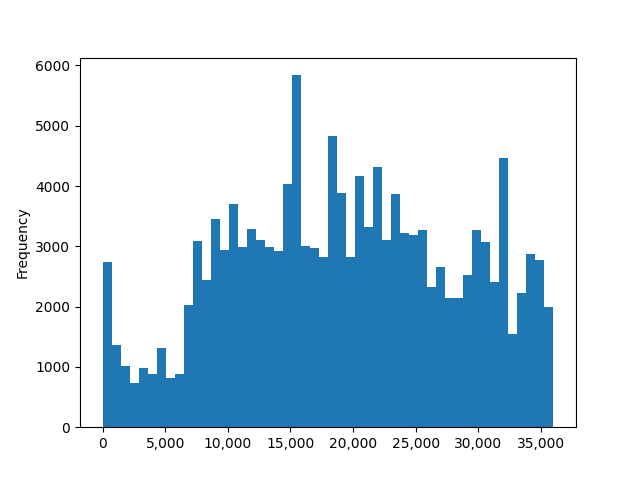
\includegraphics[width=0.90\textwidth]{../data/figures/hist_20190610_timestamps.png}
	\caption{Histogram of order update arrivals for date 20190610}
	\label{fig1}
\end{figure}

For the analysis the data will be resampled. Specifically, a grid will be used with a time interval of
100ms. This is done so as to reduce noise of the raw updates at microsecond level and detect any
signals in the data. Obviously, this grid size might cause information less and a more thorough
analysis can be done to optimize, but for practical considerations 100ms will be used as the
discretization step. 

Thus timestamps will be rounded up to the nearest 10,000 micros.
The reason to round up is to avoid look-ahead bias when using the data as a trade signal, since
rounding down will match an order update with a timepoint in the past. In addition, when
discretizing to a grid, there might an issue when there are no updates available. In that case a
forward interpolation is done by using the last known value.

\section{Feature Selection}
\subsection{Target to predict}
For the targets the following was considered:
\begin{itemize}
    \item The simple average mid price:
        \begin{equation}
            P_{mid} = \frac{bp0 + ap0}{2} \label{bbomid}
        \end{equation}
    \item The inverse volume weighted mid price:
        \begin{equation}
            P_{mid} = \frac{bp0\times aq0 + ap0 \times bq0}{bq0 + aq0}
        \end{equation}
        This mid has the benefit of taking into account the order imbalance at the top level: if
        the buy order volume is higher, the price will be skewed higher to the ask, and vice-versa
        if the sell order volume is higher.
\end{itemize}

For the target the simple average mid (equation \ref{bbomid}) is used rather than the inverse weighted mid. The reasoning
being that the inverse weighted mid is a predictor of sorts for the simple average mid.
Specifically, the target will be the mid price change time $t$ and $t+\delta$:

\begin{equation}
    V(t) = P_{mid, t+\delta} - P_{mid, t}
\end{equation}

The logic of using the price difference being that for trading predicting the price moves is more
useful than the absolute price level.

A plot of the data and some comments:
 \begin{figure}[H] 
	\centering
	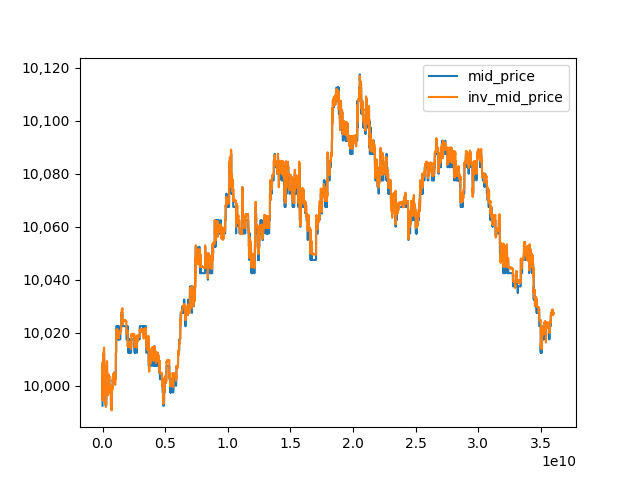
\includegraphics[width=0.90\textwidth]{../data/figures/time_series_20190610_mid_price_inv_mid_price.png}
	\caption{}
	\label{fig2}
\end{figure}

\subsection{Features}
For the features, the ones below are considerd:
\begin{itemize}
    \item The bid-offer spread calculated as:
        \begin{equation}
            S = \frac{ap0 - bp0}{P_{mid}}
        \end{equation}
    The intuition of using the spread as a predictor for the change of the mid-price is that if say
    the spread is relatively wide, then the probability of a non-markeatable limit order
    arriving whose price is inside the spread is also higher. Whereas if the bid-offer spread was very
    narrow, then the mid-price can only change when side of the order-book is depleted.
\item 
\end{itemize}



\section{Model Selection}

\section{Results}

%%\section{Conclusion}       

\bibliographystyle{plain}
%\bibliography{report_sci_comp_3}

\end{document}
